\chapter{Problemstellung}
\label{chap:problemkontext}
Wie einleitend beschrieben, existiert für den MDV-Prozess bei Mercedes-AMG bislang kein dokumentiertes bzw. modelliertes Prozessmodell. Diese Problemstellung wird im folgenden Abschnitt anhand eines Big Picture visualisiert und erläutert.
\\
Im Zertifizierungskontext des automobilen Bereichs bildet der MDV eine Schnittstelle zwischen der technischen Entwicklung, der Verbrauchs- und Reichweitensimulation, der Homologation und Marktkommunikation. Trotz dieser Schnittstellenfunktion ist der MDV-Prozess bisher nicht formalisiert dokumentiert \citeintern{amg2025mdvvorgehensweise}. Der Ablauf selbst ist in der Praxis zwar bekannt, stützt sich jedoch auf das informelle Expertenwissen einzelner Mitarbeiter und liegt bisher nicht in einer standardisierten Form vor. Wenn dieser Zustand andauert, stützt sich das Wissen über den tatsächlichen Prozessablauf weiterhin und zunehmend auf die Erfahrung einzelner Mitarbeiter. Für andere Beschäftigte ist der Ablauf dann nicht nachvollziehbar, da eine verlässliche Dokumentation als gemeinsame Wissensgrundlage fehlt. Beim Ausscheiden oder Wechsel erfahrener Mitarbeiter besteht das Risiko, dass zuvor undokumentiertes, implizites Wissen verloren geht. Dies kann zu Rollenunklarheiten und einer unsystematischen Ausführung beitragen und zugleich die Bewertung von Schwachstellen sowie eine Weiterentwicklung der Prozesse erschweren \cite{Hylko2005THANKSFT}, \cite{aspara2011documentation}, \cite{Droege2003EmployeeTA}. 

\begin{figure}[htpb]
    \centering
    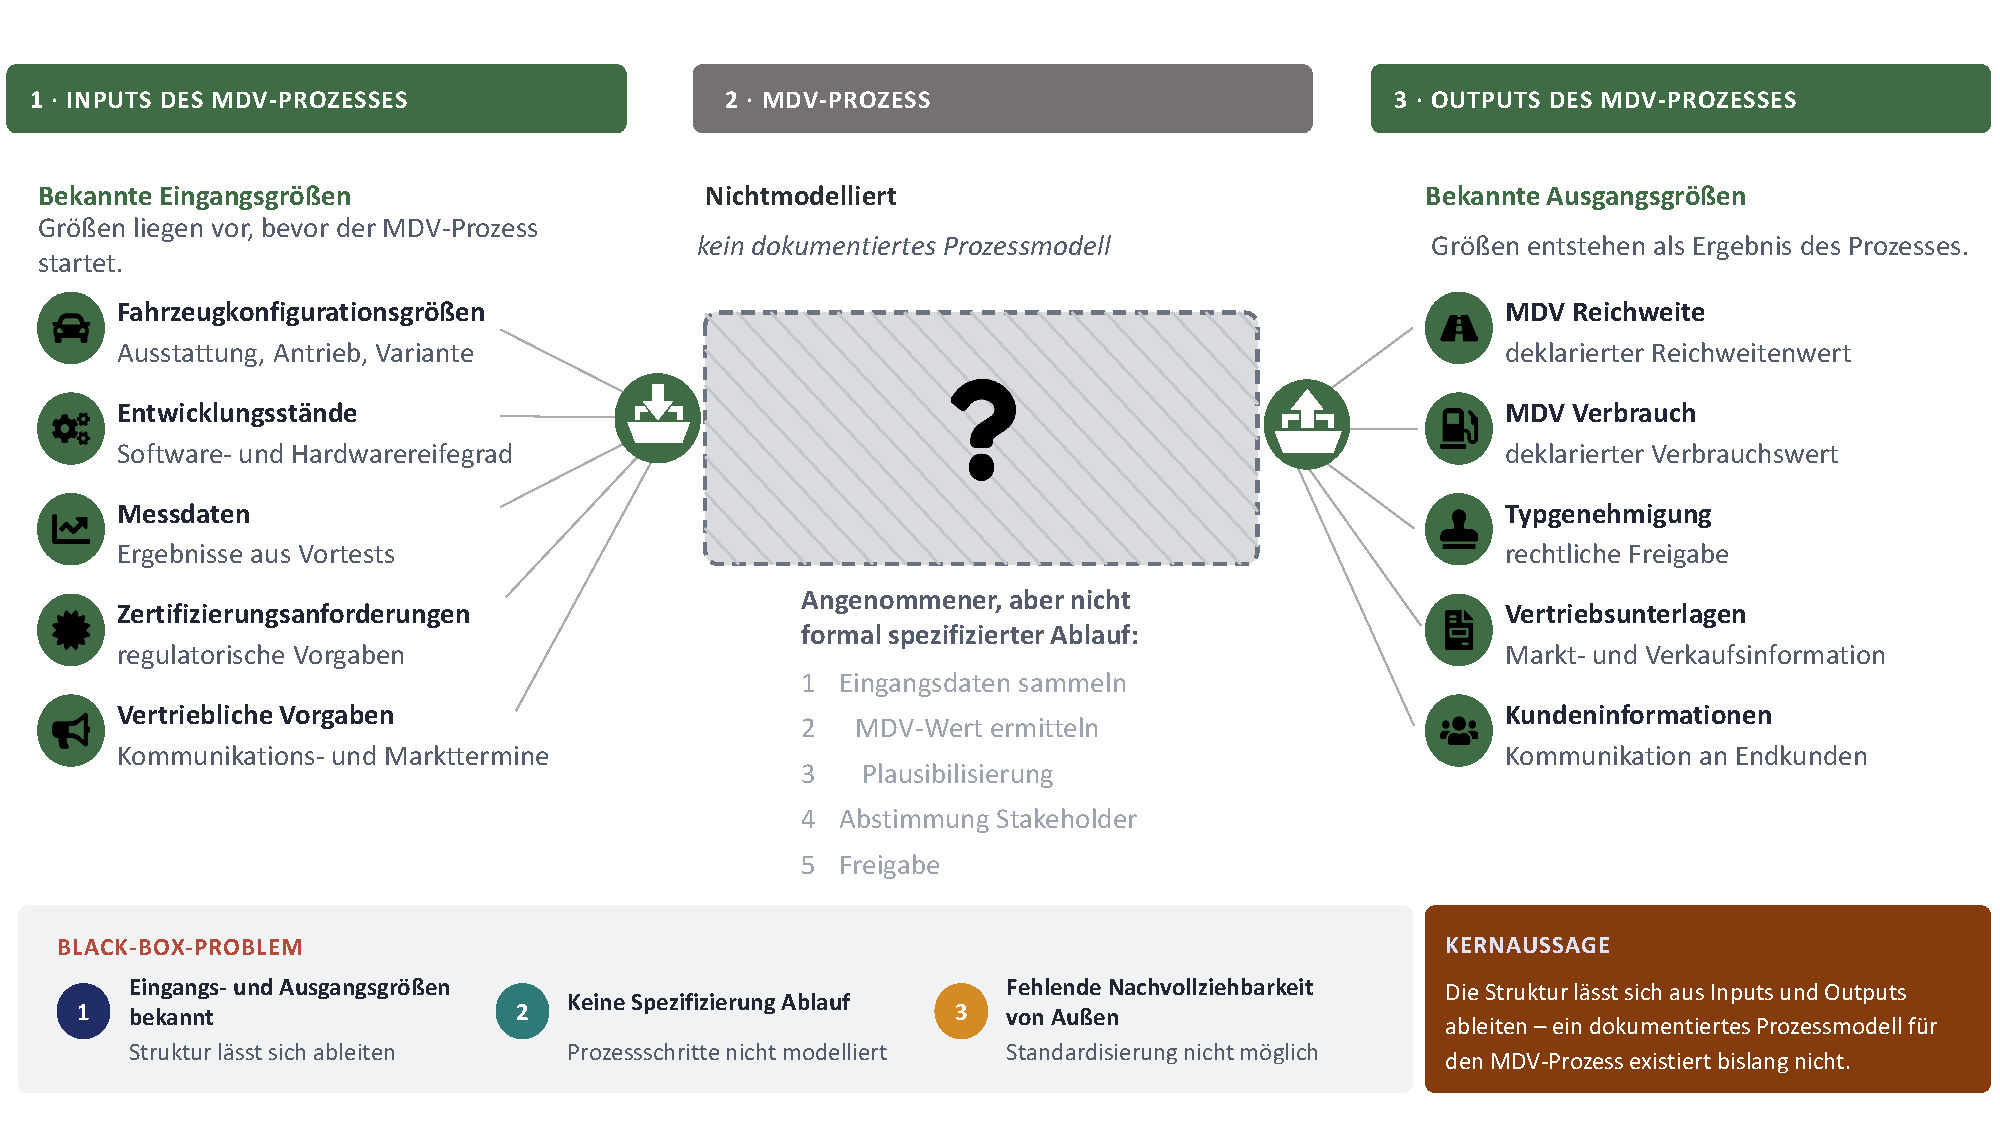
\includegraphics[width=1.0\linewidth]{images/MDV_BlackBox_Problem.pdf}
    \caption{Visualisierung des Big Picture, eigene Darstellung}
    \label{fig:bigpicture}
\end{figure}
\noindent
Das in Abbildung \ref{fig:bigpicture} dargestellte Big Picture veranschaulicht die vorliegende Problemstellung anhand der MDV-Festlegung. Die Abbildung zeigt links die bekannten Eingangsgrößen, die vor Beginn des Prozesses vorliegen. Auf der rechten Seite sind die bekannten Ausgangsgrößen abgebildet, die das Ergebnis des MDV-Ablaufs sein sollten. Das dazwischen liegende Feld wird als schraffierte Fläche dargestellt, da noch kein modelliertes Prozessmodell existiert. Die darunter angeordneten fünf Schritte sind der angenommener Ablauf, der formal nicht weiter spezifiziert wurde. Konkret umfassen die Eingangsgrößen die Fahrzeugkonfiguration, den Entwicklungsstand, vorliegende Messdaten, Zertifizierungsanforderungen sowie vertriebliche Vorgaben. Die entsprechenden Ausgangsgrößen bestehen aus dem deklarierten Reichweiten- bzw. Verbrauchswert, der Typgenehmigung, den Vertriebsunterlagen sowie den daraus abgeleiteten Kundeninformationen. Diese Gegenüberstellung zeigt, dass die Voraussetzungen und Ergebnisse des MDV-Ablaufs vorhanden sind. Die Umsetzung von Eingangs- in Ausgangsgrößen folgt jedoch keiner dokumentierten Struktur. Die im unteren Bereich der Abbildung ergänzte Zusammenfassung fasst die Kernaussage in drei Punkten zusammen. Die Struktur des Prozesses lässt sich aus den bekannten Rahmengrößen ableiten, der eigentliche Ablauf bleibt jedoch unspezifiziert. Dadurch ist eine Nachvollziehbarkeit gegenüber Prüfinstanzen sowie unternehmensinternen Stakeholdern nicht gegeben.
\\
Bei diesem Ablauf sind mehrere Fachbereiche mit jeweils eigenen Systemen und Datenbeständen beteiligt, die über die Eingangs- und Ausgangsgrößen mit dem Prozess verbunden sind. Die Herausforderung liegt nicht in den Fachbereichen selbst, sondern an der Schnittstelle zwischen ihnen und dem MDV-Ablauf sowie im Ablauf selbst. Jedem Fachbereich ist zwar bekannt, welche Größen er einbringt oder empfängt. Für die übrigen Beteiligten ist es jedoch nicht klar formal definiert welche Schritte, Verantwortlichkeiten und Entscheidungen innerhalb des Prozesses tatsächlich dazwischen liegen. Dadurch wird die Zusammenarbeit der Fachbereiche auf den reinen Austausch von Ein- und Ausgangsgrößen reduziert, ohne dass die beteiligten Parteien den dahinterliegenden Ablauf nachverfolgen können. Damit fehlt eine Grundlage für ein gemeinsames Verständnis des Prozesses und dessen Standardisierung.
\\
Neben dieser Herausforderung tragen weitere Faktoren zur Komplexität dieses Problem bei. Durch die Beteiligung mehrerer Fachbereiche mit unterschiedlichen fachlichen Blickwinkeln und Interessen erhöht sich die Anzahl aller möglichen Schnittstellen, an denen Informationslücken entstehen können. Ein weiterer Punkt ist die Heterogenität der Inputs, die aus unterschiedlichen Quellen und Systemen stammen und damit eine einheitliche Beschreibung des Prozesses erschweren. Für die verschiedenen Märkte existieren darüber hinaus jeweils eigene regulatorische Anforderungen, Zertifizierungsverfahren und Zeitschienen. Dadurch entstehen parallel mehrere marktspezifische Vorgehensweisen für die zu zertifizierenden Märkte. Eine vollständig einheitliche Ausgestaltung des Prozesses ist unter diesen Rahmenbedingungen nicht möglich, da marktspezifische Unterschiede berücksichtigt werden müssen. Daneben ist der MDV-Prozess in einen übergeordneten Rahmen eingebunden. Der \acs{WLTP}-Prozess bezeichnet bei Mercedes-AMG den internen Gesamtprozess rund um das \acs{WLTP}-Verfahren und setzt sich aus mehreren Teilprozessen der beteiligten Fachbereiche und Gewerke zusammen. Dazu gehört auch der MDV-Prozess, der innerhalb des Gesamtprozesses als Teilprozess eingebunden ist, und der derzeit an die Abgasnorm Euro 7 angepasst wird \citeintern{wltp_eu7_workshop2026}. Dementsprechend funktioniert der MDV-Prozess zwar operativ, seine innere Struktur ist von außen jedoch weder nachvollziehbar noch systematisch weiterentwickelbar. Zur Beantwortung der eingangs formulierten Forschungsfrage ist deswegen eine Methodik der Prozessaufnahme und -modellierung notwendig, mit der sich die beschriebene Black-Box-Problematik auflösen lässt. Diese Methodik wird im folgenden Kapitel vorgestellt.




%TODO




% Die Forschungsfrage nennt Prozesstransparenz. Das Fazit sagt „nachvollziehbar“ und „erstmals als gemeinsame Grundlage nach Freigabe“, prüft aber weder Entscheidungen noch Prüfinstanzen aus Kap. 2. Entscheidungen werden zu „Vorgehen“ abgeschwächt.

